\chapter{Introduction}
\section{Background}
The electromagnetic radio spectrum is a natural resource that remains 
underutilized \cite{haykin05}.
It is licensed by governments for use by transmitters and receivers.
With the explosive proliferation of cell phones and other wireless 
communication devices,
we cannot afford to waste our spectral resources anymore.

In November 2002, the Spectrum Policy Task Force, a group under the Federal
Communications Commission(FCC) in the United States, published a report saying
\cite{repFCC}, 
\begin{quote}
``In many bands, spectrum access is a more significant problem than physical 
scarcity of spectrum, in large part due to legacy command-and-control 
regulation that limits the ability of potential spectrum users to obtain such 
access.''
\end{quote}

If we were to scan the radio spectrum even in metropolitan places where it's
heavily used, 
we would find that \cite{staple04}:
\begin{enumerate}
	\item some frequency bands are unoccupied most of the time,
	\item some are only partially occupied and
	\item the rest are heavily used.
\end{enumerate}

\begin{figure}
\centering
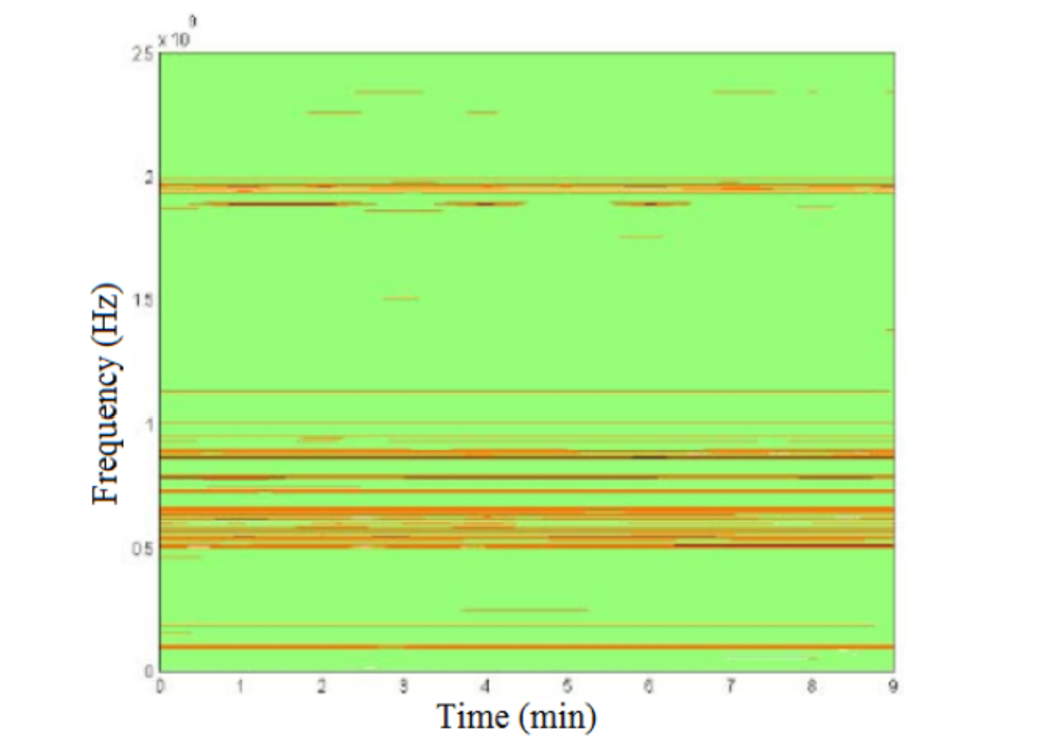
\includegraphics[width=0.7\textwidth]{../images/freqUsage}
\caption{Frequency usage of the Spectrum}
\label{freqUsage}
\end{figure}

The underutilization of spectral resources leads us to think in terms of 
\emph{spectrum holes}, which are defined as \cite{kolodzy01}:
\begin{quote}
\emph{A spectrum hole is a band of frequencies assigned to a primary user, 
but, at a particular time and specific geographic location, the band is not 
being utilized by that user.
}
\end{quote}

The spectrum can be better utilized by enabling secondary users (users who are
not licensed to use the services) to access spectrum holes unoccupied by 
primary users at the location and the time in question. 
\emph{Cognitive Radio}, which includes software-defined radio, has been 
promoted as the means to make efficient use of the spectrum by exploiting the 
existence of spectrum holes \cite{haykin05}\cite{mitola99}\cite{mitola00}.

\section{Cognitive Radio}
One of the definitions of Cognitive Radio is \cite{haykin05}:
\begin{quote}
\emph{Cognitive radio is an intelligent wireless communication system that is
aware of its surrounding environment (i.e., outside world), and uses the 
methodology of understanding-by-building to learn from the environment and 
adapt its internal states to statistical variations in the incoming RF stimuli
by making corresponding changes in certain operating parameters (e.g., 
transmit-power, carrier-frequency, and modulation strategy) in real-time, with
two primary objectives in mind:
\begin{itemize}
	\item highly reliable communications whenever and wherever needed;
	\item efficient utilization of the radio spectrum.
\end{itemize}}
\end{quote}

Besides, a cognitive radio is also reconfigurable. This property of cognitive 
radio is provided by a platform known as \emph{software-defined radio}. 
Software-defined Radio (SDR) is basically a combination of two key 
technologies: digital radio, and computer software.

\section{Contribution of Thesis}

A cognitive base transceiver station is developed to demonstrate the efficient 
utilization of spectrum by allowing secondary users to make use of the 
frequency bands that are already licensed to primary users but that are not 
being used at that particular time and space.

\begin{enumerate}
    \item A two-frequency system is developed where as soon as the presence of 
    primary users is detected in $F_1$  the secondary BTS switches from $F_1$ 
    to $F_2$ and vice-versa.
    \item The two-frequency system is extended to a four-frequency one where
    two of the four frequency channels always remain occupied. The secondary
    system switches to one of the two unused frequency channels.
    \item For sensing the frequency channels the energy detection based
    spectrum sensing method has been used and for peak detection the method 
    called CUSUM has been used. The frequency used by the secondary users is
    sensed continuously and as soon as the presence of primary users in that 
    frequency is detected the secondary finds an underutilized frequency 
    nearby and switches to that frequency.  
\end{enumerate}



\section{Organization}
The remaining chapters of this document are organized as follows. Chapter 2 
briefly touches upon the GSM system architecture and the GSM protocol 
architecture. Chapter 3 introduces Software Defined Radio (SDR) and some of the
tools that make SDR possible like the Universal Software Radio Peripheral 
(USRP N210) and the GNU Radio software package. Various parts of the OpenBTS 
software are described in Chapter 4. Chapter 5 reviews various techniques of 
spectrum sensing and gives a comparison among them. Chapter 6 describes the 
Cognitive Radio (CR) testbed that we developed using OpenBTS. Flowgraphs of
the algorithms developed while making the CR testbed are also given in
Chapter 6. Finally, Chapter 7 concludes this document.
